\chapter{小世界复杂网络的混沌、同步动力学}
本章针对一种新型的Duffing-WS型小世界网络,首先利用变分法推导其最大李雅普诺夫指数表达式,并以李雅普诺夫指数作为混沌现象的判断标准研究该复杂网络的混沌现象,
同时讨论了网络混沌现象对网络各个参数的依赖关系。接着分析同步。。。。
研究表明,Duffing-WS型小世界网络具有比单个Duffing-方程更为复杂的混沌特性。。。
\section{Duffing-WS型小世界网络基本模型}

Duffing 方程作为研究最为充分的混沌连续动力系统模型之一,具有丰富的非线性动力学行为 [15]。
早在1918年,Duffing 首次引入Duffing 方程用来描述机械问题中具有硬弹簧效应的非线性振子。后来到1979年,牧恩(Moon)和霍尔姆斯(Holmes)将其修改为描述处在两个永久磁铁非均匀场中的支架梁的强迫振动。一般的Duffing 振子可由如下的方程描述:
\begin{equation}
    \ddot{x}+\gamma \dot{x}+\partial V(x)/\partial x = f(t)
\end{equation}
其中, $\gamma>0$为阻尼系数,$V(x)$表示物体所受势场力,$f(t)$表示外激励力。当$V(x)$和$f(t)$取不同的形式时,便可得不同形式的Duffing方程。

规范化的 Holmes型 Duffing 方程如下:
\begin{equation}
    \ddot{x}=-\gamma \dot{x}+a x-b x^{3}+A \sin (\Omega t)
\end{equation}
令$y=\dot{x}$,则上述方程可以改写为:
\begin{equation}
\left\{
  \begin{array}{ll}
    \dot{x}=y, \\
    \dot{y}=a x-b x^{3}-\gamma y+A \sin (\Omega t),
  \end{array}
\right.
\end{equation}

当周期振幅为0时,通过令方程组(*)右式为0可得Holmes型 Duffing 方程(*)具有三个平衡点:$S=(0,0),F_1=\left(\sqrt{\frac{a}{b}},0\right),F_2=\left(-\sqrt{\frac{a}{b}},0\right)$。
其中$F_1,F_2$是稳定的焦点,而$S$是不稳定的鞍点。

此外,它的相空间体积为:
\begin{equation}
div V = \frac{\partial y}{\partial x}+\frac{\partial(a x-b x^{3}-\gamma y)}{\partial y} = -\gamma <0
\end{equation}
所以上述Duffing系统是一个耗散动力系统。

当外加周期驱动力不存在(即$A=0$)时,受迫的Holmes型 Duffing方程(*)
退化为无摄动的Duffing方程,方程的解$x\left(t\right)$将以螺旋形式(衰减振荡)趋于两稳定焦点之一,并且初始条件决定着系统将最终趋于哪一焦点。
在其他参数固定的条件下,周期驱动力的幅值A从0开始逐渐增加到1时,方程的解会经历同宿轨道、分岔、混沌和大尺度周期等各个状态。
图 *给出了当$A$取不同值时 Duffing 方程输出响应的时域图,图*则给出了其输出的相图,展示了Duffing 振子从吸引子状态,再通过倍周期分岔走向混沌的过程。
 \begin{figure}[!htbp]
    \centering
    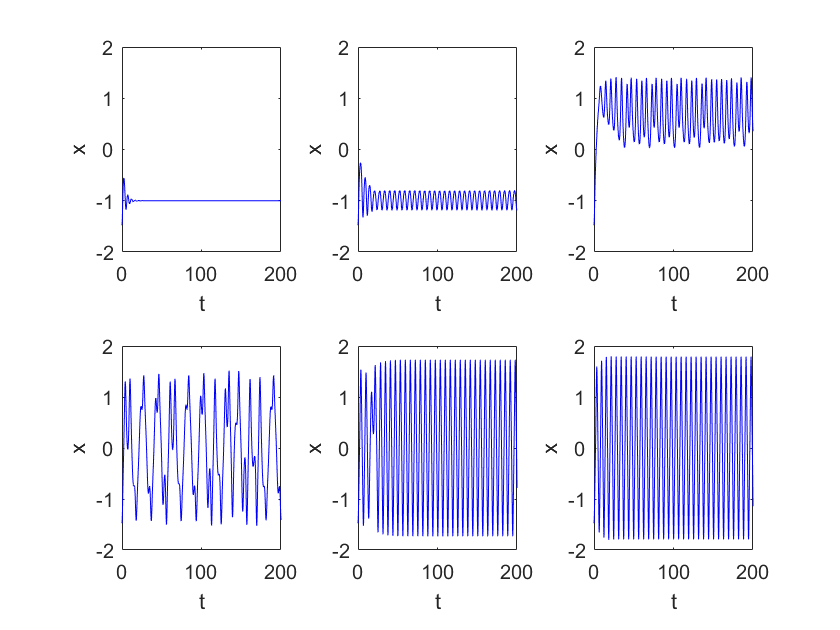
\includegraphics[width=0.9\textwidth]{duffingtime.png}\caption{不同周期振幅$A$取值时,Duffing 方程输出时域图}
 \end{figure}

 \begin{figure}[!htbp]
    \centering
    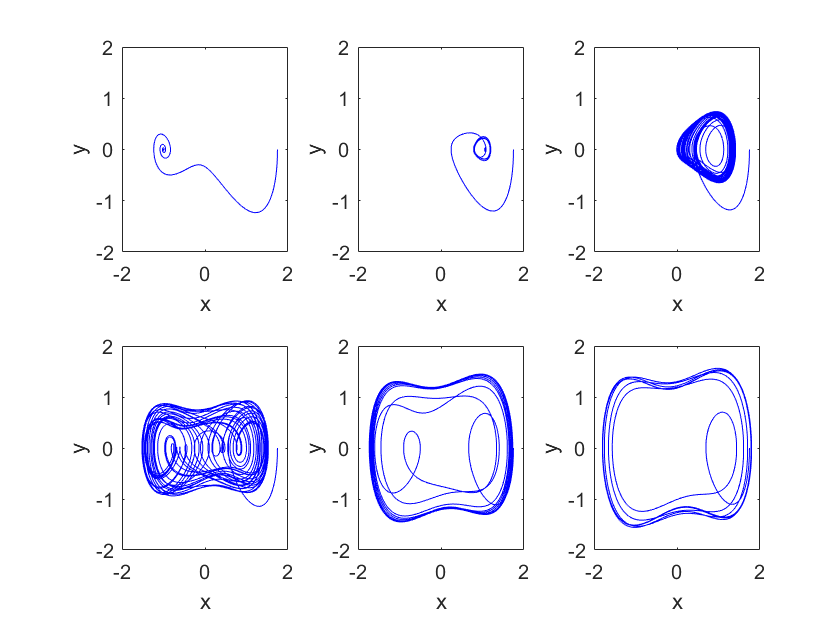
\includegraphics[width=0.9\textwidth]{duffingphase.png}\caption{不同周期振幅$A$取值时,Duffing 方程输出相图}
 \end{figure}

所谓分岔是指对于含参数的系统,当参数变动并经过某些临界值时,系统的定态性质
(如平衡状态或者周期运动的数目和稳定性)会发生突然的变化。分岔图则绘制了系统的庞加莱截面输出随参数的变化图,
可用于比较微小参数扰动对系统指标的影响,是系统稳定性的直观衡量。 下图*给出了Duffing 方程输出$x$随周期驱动幅度$A$变化的分岔图(借助庞加莱截面),
也可以看到随着周期驱动幅度$A$的变化,Duffing 方程从吸引子走向混沌、大周期运动的过程。
 \begin{figure}[!htbp]
    \centering
    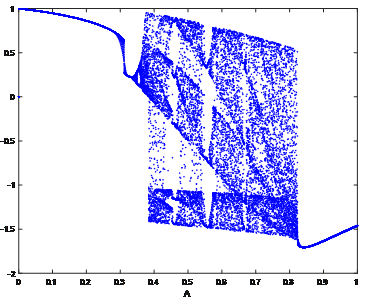
\includegraphics[width=0.7\textwidth]{30.png}\caption{Duffing 方程随周期振幅$A$变化的分叉图}
 \end{figure}

\subsection{Duffing-WS型小世界网络基本模型}

基于上述经典的Holmes型 Duffing 方程(3.1),本文提出如下具有N个节点的以WS小世界网络方式进行连接的Duffing复杂网,即Duffing- WS型小世界网络,其动力学方程为:
\begin{equation}
    \ddot{x}_{i}=-\gamma \dot{x}_{i}+a x_{i}-b x_{i}{ }^{3}+\varepsilon \sum_{j=1}^{N} a_{i j}\left(x_{j}-x_{i}\right)+A \sin (\Omega t), i=1,2, \ldots, N
\end{equation}
其中,$x_i(t)$为第$i$个节点的输出状态变量, $i=1,2,\ldots,N$。$A\sin(\Omega t)$为周期驱动力, 
$\varepsilon \sum_{j=1}^{N} a_{i j}\left(x_{j}-x_{i}\right)$表示其它节点对第$i$个节点的耦合作用项, 称为耦合项,$\varepsilon$为网络耦合强度,
$\left(a_{ij}\right)_{N\times N}$为网络的邻接矩阵。一般的,对于一个无权无向的简单连通网络来说,
如果第$i$个节点和第$j$个节点之间有连接,则$a_{ij} = 1$;否则$a_{ij} = 0$。

这里我们采用Watts 和 Strogatz 提出的WS小世界网络作为网络连接拓扑结构[3],其连接方式按如下方式进行:

(1)首先, $N$个节点连接形成一个规则的相邻网络,每个节点与它最近邻的$K$个节点相连,这里$K$称为重连度;
(2)而后以概率$p$ (称为重连概率)随机地重新连接网络中的每条边,
即将边的一个端点保持不变, 而另一个端点取为随机选择的一个节点, 且规定任意两个不同的节点之间至多只能有一条边, 每一个节点都不能有边与自身相连。

对于WS小世界网络而言,当$p = 0$,模型为规则网;当$p = 1$时则为随机网;当$0 < p < 1$,则得到介于规则网与随机网之间的小世界网络。

图*给出了节点数为$N=50$,连接度为$K = 4$,重连概率$p = 0.5$的Duffing-WS型小世界网络的连接拓扑结构图。
\begin{figure}[!htbp]
   \centering
   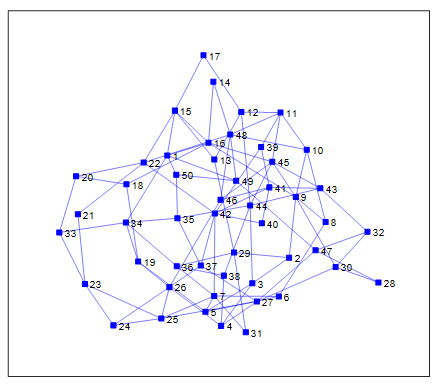
\includegraphics[width=0.6\textwidth]{WStop.png}\caption{Duffing-WS型小世界网络的连接拓扑结构图}
\end{figure}
通过引入Laplacian矩阵为$L=\left(l_{ij}\right)_{N\times N},l_{ij}=\begin{cases}
    -a_{ij},i\neq j \\ \sum_{j\neq i}a_{ij},i=j
\end{cases}$,则方程(3.2)可以改写为如下形式:
\begin{equation}
    \ddot{x}_{i}=-\gamma \dot{x}_{i}+a x_{i}-b x_{i}^{3}+A \sin (\Omega t)-\varepsilon\sum_{j=1}^{N} l_{i j} x_{j}
\end{equation}
由Laplacian矩阵的性质可知,$L$是一个实对称的弱对角占优矩阵,且对角元均非负,所以是半正定的。
事实上,复杂网络的邻接矩阵或Laplacian矩阵全面地刻画了网络节点之问的相互关系,其特征值和特征向量则揭示了网络拓扑及其整体行为的信息。

\section{Duffing-WS型小世界网络基本动力学特性研究}
\subsection{分岔图分析}
我们的研究发现,当驱动力幅度A值在(0,1)范围变化时,随着A值的变化,Duffing-WS小世界网络的各个粒子输出也将呈现小尺度周期运动、
我们的研究发现,当驱动力幅度$A$值在(0,1)范围变化时,随着$A$值的变化,Duffing-WS小世界复杂网络(*)的各个节点输出也将呈现小尺度周期运动、
倍周期分岔、混沌和大尺度周期运动等状态。我们首先借助庞加莱截面给出Duffing-WS小世界网络的分岔图。 分岔图绘制了系统的庞加莱截面输出随参数的变化图,可用于比较微小参数扰动对系统指标的影响,
在本文中用来衡量混沌现象。

取庞加莱截面为$t=j T, T=2 \pi / \Omega$,在此截面上引入如下宏观变量$\sigma(j T)$来描述系统的集体行为:
\begin{equation}
    \sigma(j T)=\frac{1}{N} \sum_{i=1}^N x_i(j T)
\end{equation}
图(a)中给出了借助庞加莱截面单个 Duffing 方程的解随驱动力幅度 $A$ 变化的分岔图。图 (b) 给出了借助 $\sigma(j T)$, 
节点个数为 $N=100$ 的 Duffing-WS 型 小世界网络关于幅度 $A$ 的变化的分岔图。和图 1 中单个 Duffing 方程关于幅度 $A$ 
的分岔图对比可知, Duffing-WS 型小世界网络的分岔图事实上也历经了小尺度 周期运动、倍周期分岔、混沌和大尺度周期运动等状态,
 在大尺度周期状态之 后又进入了短暂的混沌状态, 因此其分岔图具有更为复杂的特性。
 \begin{figure}[!htbp]
    \centering
    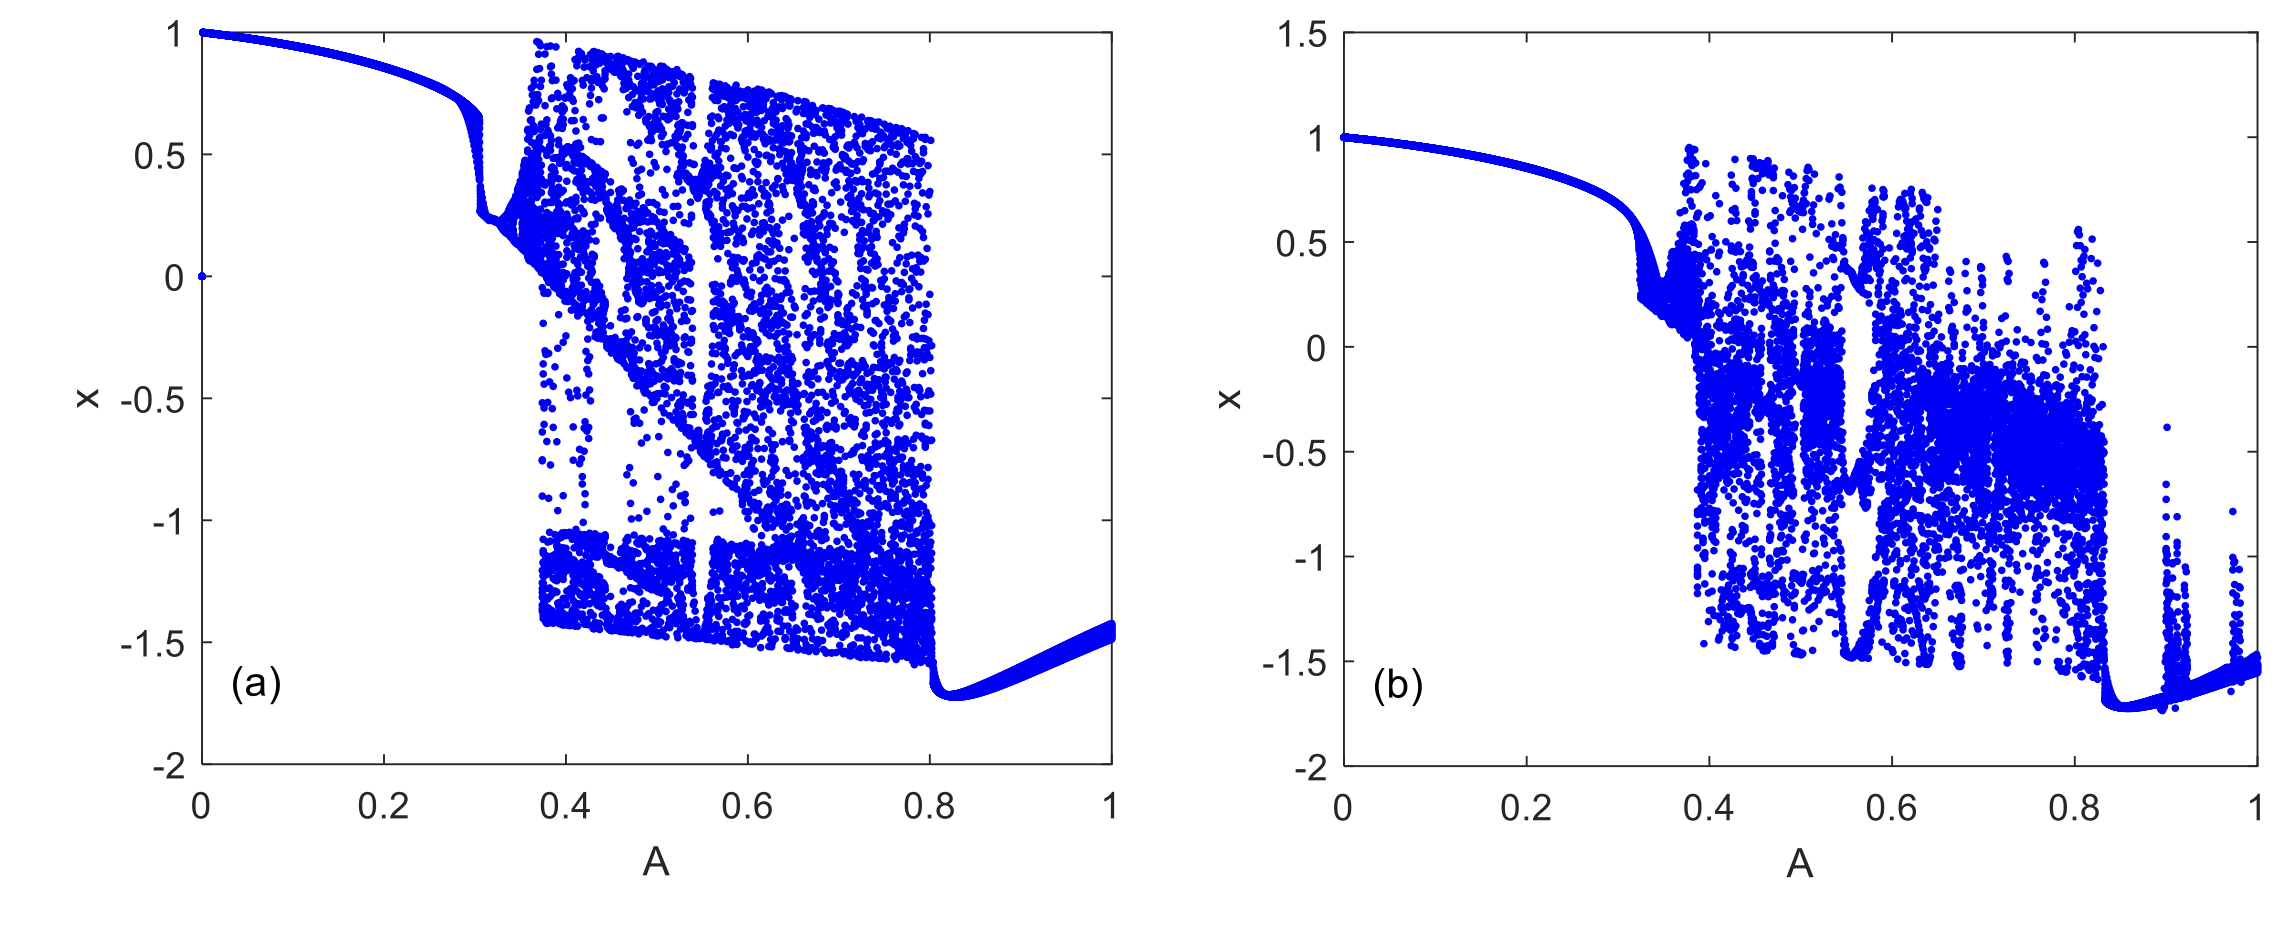
\includegraphics[width=0.8\textwidth]{31.png}
 \end{figure}
\subsection{基于最大李雅普诺夫指数的混沌动力学分析}
从3.1节可以看出,通过分岔图并不容易定量分析复杂系统的混沌行为,而对耦合系统混沌进行分析的另外一个指标为系统的最大Lyapunov指数
(LE指数)。LE指数是衡量系统动力学特性的一个重要定量指标,表现了系统在相空间中相邻轨道间收缩或发散的平均指数率。

这一节我们利用变分法推导 Duffing-WS 型小世界网络的最大 LE 指数表 达式, 利用最大 LE 指数来研究其混沌现象,
并分析小世界网络重连度 $K$, 重连 概率 $p$ 和耦合强度 $\varepsilon$ 等对复杂系统处于混沌运动状态参数范围的影响。
其中,LE指数采用数值模拟的方式给出,其计算方法的理论依据已在第二章给出。
通过令
\begin{eqnarray*}
z_i=\Omega t,\left. z_i\right|_{t=0}=0
\end{eqnarray*}
可将Duffing-WS 型小世界网络模型(*)的非自治方程变成如下的自治方程组:
 \begin{equation}
    \left\{\begin{array}{l}
    \dot{x}_i=y_i \\
    \dot{y}_i=-\gamma y_i+a x_i-b x_i^3+A \sin \left(z_i\right)-\varepsilon \sum_{j=1}^N l_{i j} x_j \\
    \dot{z}_i=\Omega
    \end{array}\right.
\end{equation}
假设 $s(t)$ 是单个 Duffing 方程(1)的解, 引入变分:
\begin{equation}
    \delta_{x i}=x_i(t)-s(t), \delta_{y i}=y_i(t)-\dot{s}(t),
\end{equation}
并结合自治方程组(*)可得到 Duffing-WS 小世界网络的变分方程为:
\begin{equation}
    \left\{\begin{array}{l}
    \dot{\delta}_{x i}=\delta_{y i} \\
    \dot{\delta}_{y i}=-\gamma \delta_{y i}+a \delta_{x i}-3 b x_i^2 \delta_{x i}+A \cos \left(z_i\right) \delta_{z i}-\varepsilon \sum_{j=1}^N l_{i j} \delta_{x j} \\
    \dot{\delta}_{z i}=0
    \end{array}\right.
\end{equation}
在不失去普遍性的情况下, 在上述变分方程中令集合 $\delta_{z i}=0$, 则变分方程可以简化为:
\begin{equation}
    \left\{\begin{array}{l}
    \dot{\delta}_{x i}=\delta_{y i} \\
    \dot{\delta}_{y i}=-\gamma \delta_{y i}+a \delta_{x i}-3 b x_i^2 \delta_{x i}-\varepsilon \sum_{j=1}^N l_{i j} \delta_{x j}
    \end{array}\right.
\end{equation}
则根据定义,本章所提Duffing-WS型小世界网络的最大LE指数表达式为:
\begin{equation}
    \lambda_{\max }=\lim _{T \rightarrow \infty} \frac{\log \left(\sqrt{\sum_{i=1}^N\left|\delta_{x i}(T)\right|+\left|\delta_{y i}(T)\right|}\right)}{T}
\end{equation}
在下面的章节中,我们利用上式计算不同参数情况下的Duffing- WS型小世界网络平均最大LE指数关于周期幅度变化的曲线,
其中LE指数大于0的区域被视为系统处于混沌运动的区域。网络的粒子个数固定为$N=100$,每条曲线均是对50个样本轨道平均后所得。
Duffing方程中的参数固定为$a=1,b=1,\gamma=0.5,\Omega=1$。此外,本文Duffing- WS型小世界网络(*)及其对于变分方程组(*)
的数值模拟均基于我们在第*节给出的微分方程四阶龙格库塔算法。
\subsection*{耦合强度$\varepsilon$对混沌的影响}
图(a)-(c)给出了不同的耦合强度 $\varepsilon$ 下平均最大 LE 指数随幅度 $A$ 变化的曲线, 重连概率均为 $p=0.5$ 。
在图(a)中 $K=2$, 当耦合强度 $\varepsilon$ 较小时 (如 $\varepsilon=0,0.2,0.4)$, 随着 $\varepsilon$ 的增大,
LE 指数大于 0 的混沌区域扩大; 当耦合强度 $\varepsilon$ 较大时 (如 $\varepsilon=$ $0.6,0.8,1,2)$, 
随着 $\varepsilon$ 的增加, LE 指数大于 0 的混沌区域则逐渐收缩, 混沌受到抑制。在这种情况下, 
由于重连度非常小节点之间的连接程度不够, 小的耦合强 度的增强反而增强系统的混沌运动; 而只有耦合强度大到一定程度, 
更大的耦合强度使得系统协同性增强, 才能抑制系统的混沌运动。\par
在图(b)中 $K=20$, 可以看到, 当 $\varepsilon=0$ 时, 小世界网络退化成独立的 $N$ 个 Duffing系统, 此时混沌区域最大, 
而当 $\varepsilon>0$ 时, 小世界网络各个节点之间存在 耦合作用, 网络的混沌区域收缩; 而此时由于重连度 $K$ 值较大, 平均 LE 指数随
幅度 $A$ 变化的曲线在不同的耦合强度 $\varepsilon$ 下基本一致, 也就是说此时小世界网络的混沌运动区域对耦合强度 
$\varepsilon$ 具有鲁棒性。同样, 在图(c)中 $K=48$, 可以看到, 随着 $\varepsilon$ 增加, 混沌区域的变化同样不明显。
综上可以看到, 和传统的规则网络不同, 本文所提 Duffing-WS 型小世界网络的耦合强度 $\varepsilon$ 
对混沌区域的影响并不是线性的, 当重连度 $K$ 较小时, 随着耦合强度的增加混沌区域呈现出先扩大后缩小的变化, 
$K$ 较大时 $\varepsilon$ 的增强对混沌区域影响不明显。\par
\begin{figure}[!htbp]
    \centering
    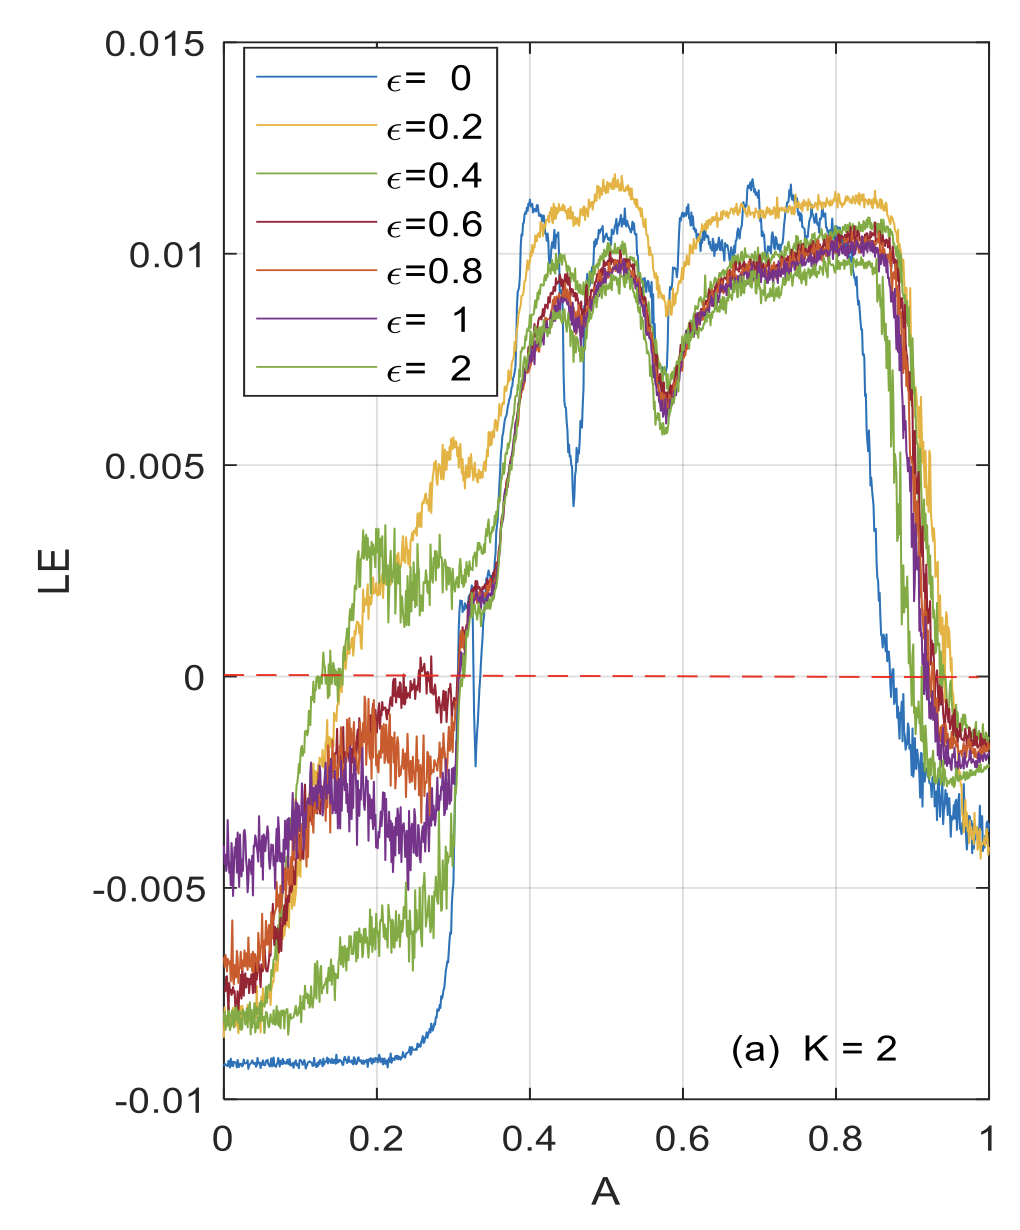
\includegraphics[width=0.5\textwidth]{k2.png}
\end{figure}
在图(a)中 $K=2$, 当耦合强度 $\varepsilon$ 较小时 (如 $\varepsilon=0,0.2,0.4)$, 随着 $\varepsilon$ 的增大,
LE 指数大于 0 的混沌区域扩大; 当耦合强度 $\varepsilon$ 较大时 (如 $\varepsilon=$ $0.6,0.8,1,2)$,
随着 $\varepsilon$ 的增加, LE 指数大于 0 的混沌区域则逐渐收缩, 混沌受到抑制。在这种情况下,
由于重连度非常小节点之间的连接程度不够, 小的耦合强 度的增强反而增强系统的混沌运动; 而只有耦合强度大到一定程度,
更大的耦合强度使得系统协同性增强, 才能抑制系统的混沌运动。\par
\begin{figure}[!htbp]
    \centering
    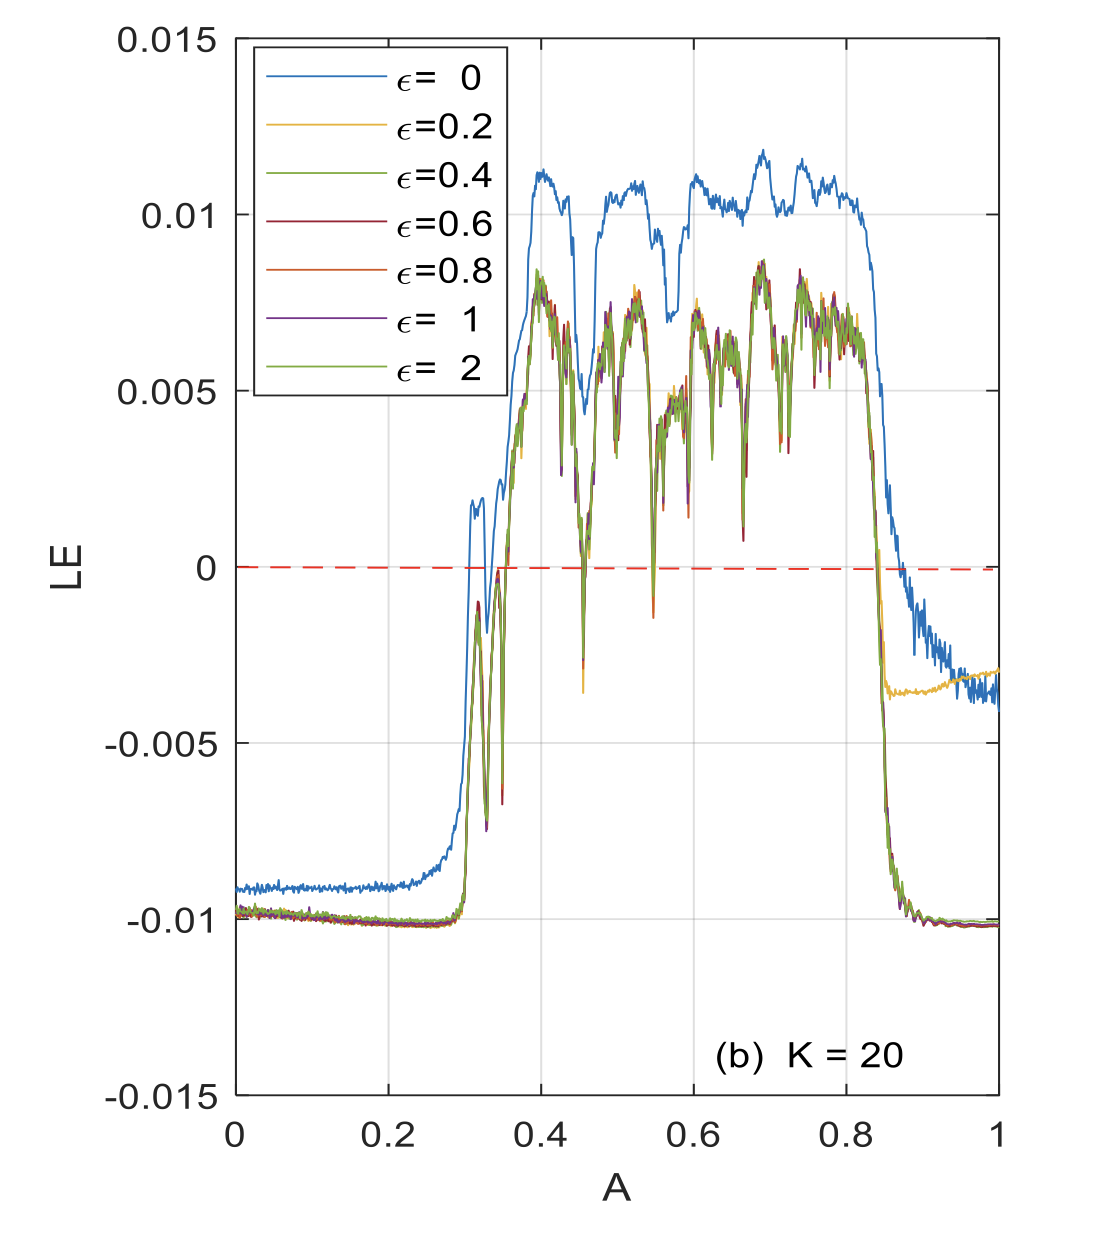
\includegraphics[width=0.6\textwidth]{k20.png}
\end{figure}

在图(b)中 $K=20$, 可以看到, 当 $\varepsilon=0$ 时, 小世界网络退化成独立的 $N$ 个 Duffing系统, 此时混沌区域最大,
而当 $\varepsilon>0$ 时, 小世界网络各个节点之间存在 耦合作用, 网络的混沌区域收缩; 而此时由于重连度 $K$ 值较大, 平均 LE 指数随
幅度 $A$ 变化的曲线在不同的耦合强度 $\varepsilon$ 下基本一致, 也就是说此时小世界网络的混沌运动区域对耦合强度
$\varepsilon$ 具有鲁棒性。\par
\begin{figure}[!htbp]
    \centering
    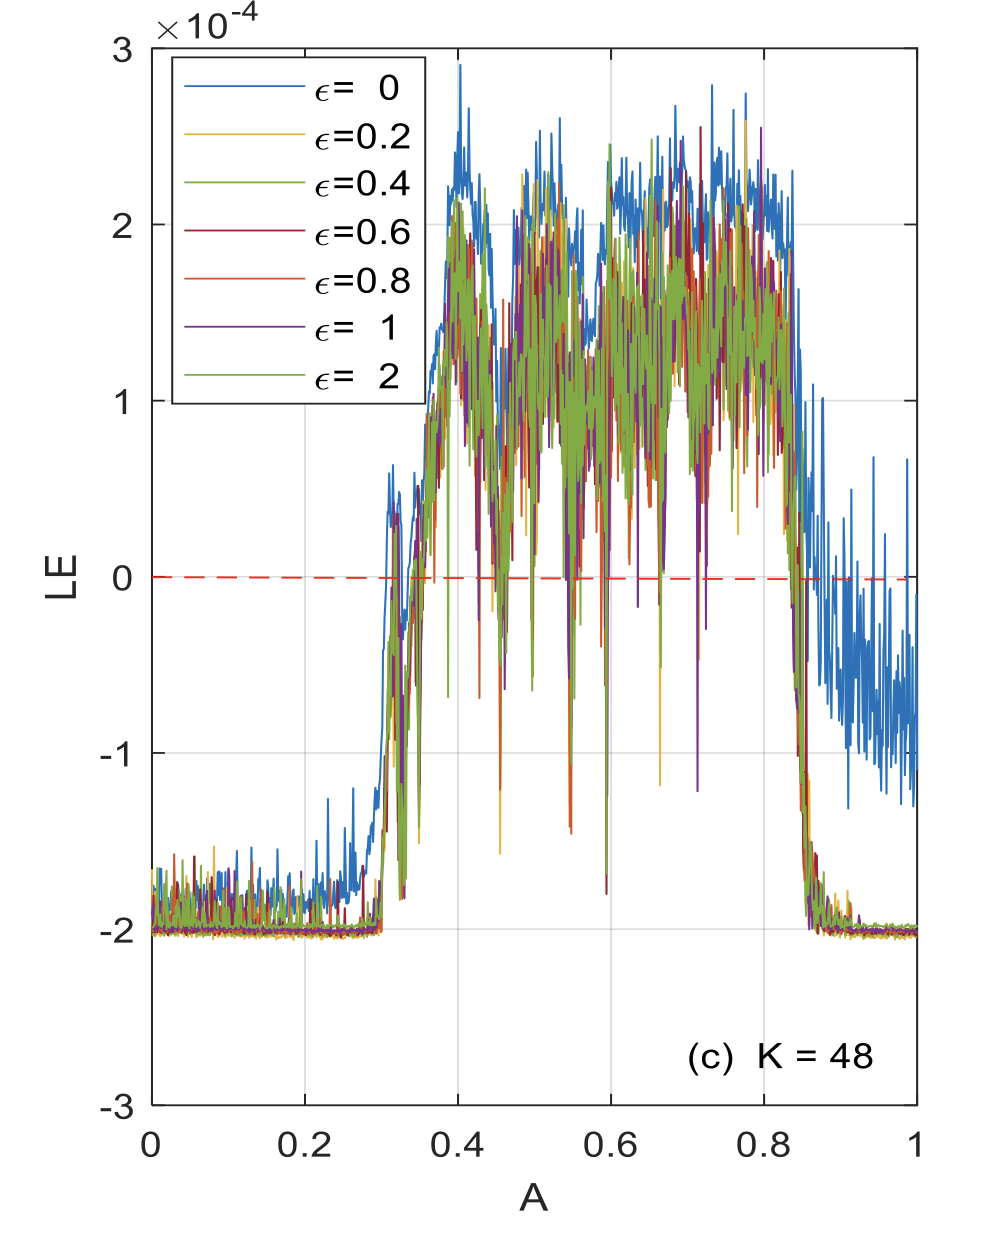
\includegraphics[width=0.5\textwidth]{k48.png}
\end{figure}
同样, 在图(c)中 $K=48$, 可以看到, 随着 $\varepsilon$ 增加, 混沌区域的变化同样不明显。
综上可以看到, 和传统的规则网络不同, 本文所提 Duffing-WS 型小世界网络的耦合强度 $\varepsilon$
对混沌区域的影响并不是线性的, 当重连度 $K$ 较小时, 随着耦合强度的增加混沌区域呈现出先扩大后缩小的变化,
$K$ 较大时 $\varepsilon$ 的增强对混沌区域影响不明显。


\subsection*{重连度$K$对混沌的影响}
我们接着分析重连度$K$对Duffing- WS型小世界网络混沌现象的影响。图(a)-(c)给出了不同的重连度 $K$ 下平均 LE 指数随幅度 $A$ 变化的曲线, 耦合强度均为 $\varepsilon=0.5$ 。\par
\begin{figure}[!htbp]
    \centering
    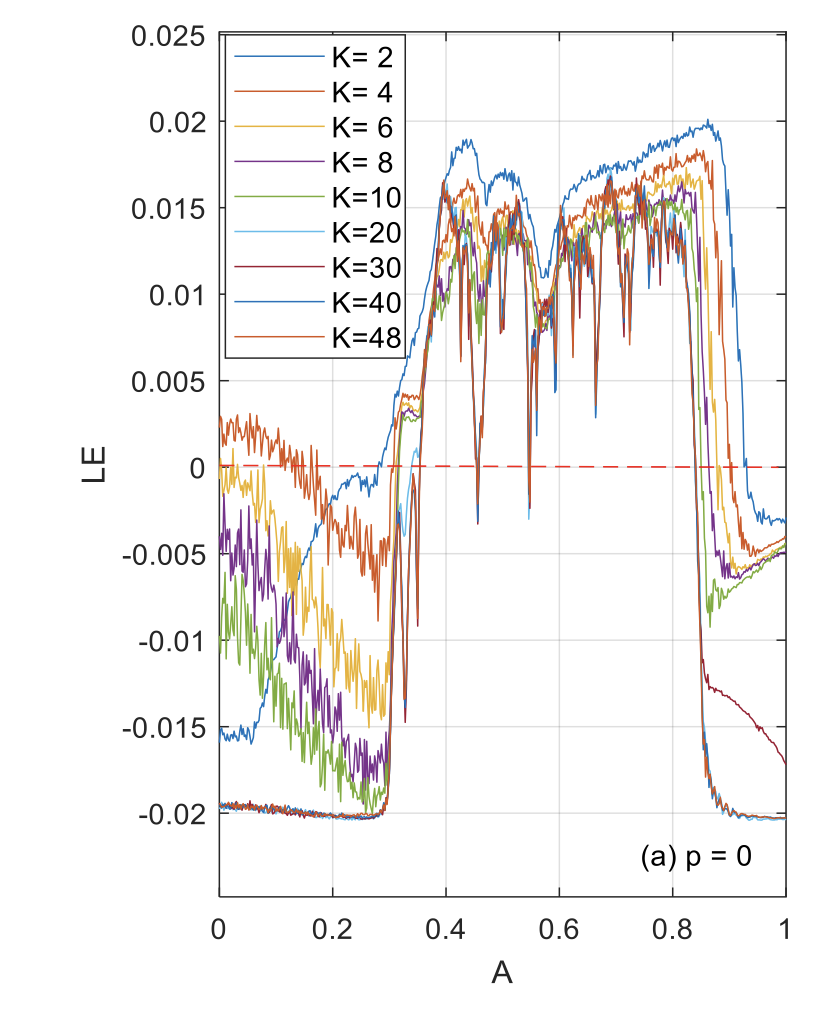
\includegraphics[width=0.5\textwidth]{pa.png}
\end{figure}
可以看出, 在图(a)中 $p=0$, 耦合网络为规则的最近邻耦合 网络, 当重连度 $K$ 较小时 $(K=2,4,6,8,10)$,
随着重连度 $K$ 的增加, LE 指数大于 0 的混沌区域先扩大再收缩, 当 $K=4$ 时混沌区域达到最大; 随后,
随着重连度 $K$ 增加到一定程度以后 $(K=20,30,40,48)$, 混沌区域随着 $K$ 值的增加而有略微地缩小,
但总体上差异不大。这说明对于规则网络, 只有足够大的重连度才会抑制 系统混沌, 较小的重连度反而增加系统的混沌运动。\par
\begin{figure}[!htbp]
    \centering
    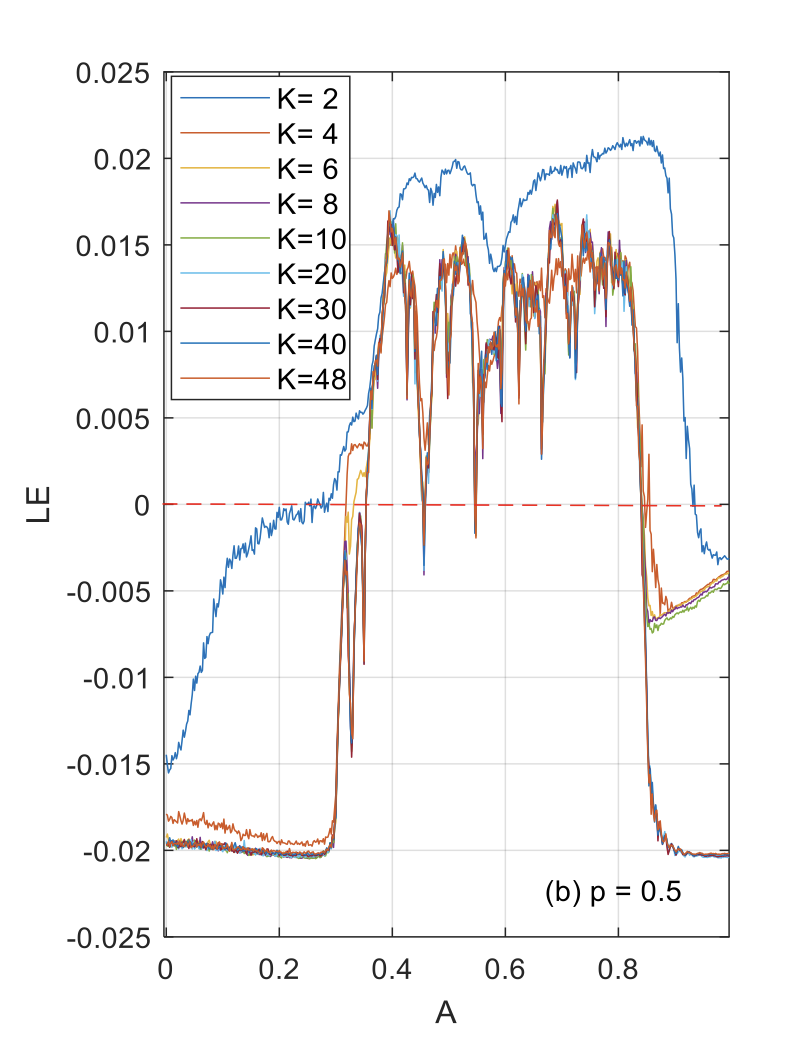
\includegraphics[width=0.5\textwidth]{pb.png}
\end{figure}
在图(b)中 $p=0.5$, 此时网络为标准的小世界模型。 $K=2$ 与$K$ 值 LE 曲线 有显著不同, 所对应的混沌区域最大,
LE 指数在各个振幅处的值都最高, 可见 重连度 $K$ 较低时更容易产生较大的混沌范围。 $K=4,6$ 比起 $K=2$ 的 LE 曲线, 其
大于 0 的区域明显缩小, 即重连度的增加明显抑制了网络混沌运动; 随着 $K$ 值进 一步增加, 系统 LE 曲线几乎没有变化,
这是因为当重连度足够高时, 系统各节 点输出间差异很小, 混沌区域几乎一致。\par
\begin{figure}[!htbp]
    \centering
    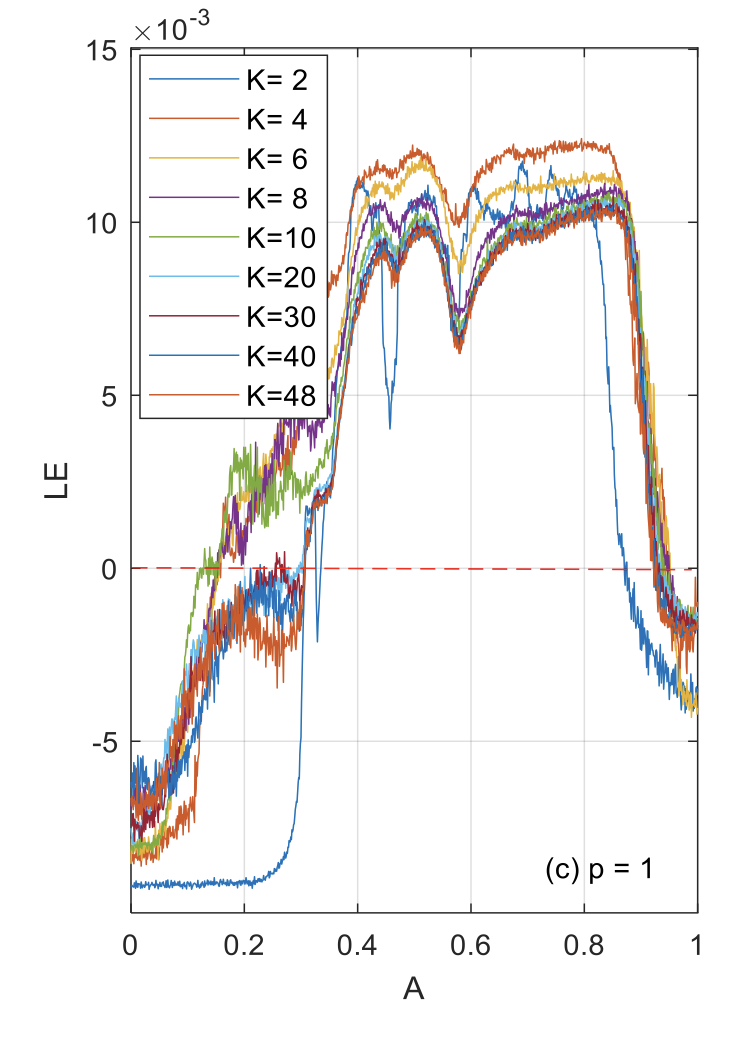
\includegraphics[width=0.45\textwidth]{pc.png}
\end{figure}
在图 (c)中 $p=1$, 此时网络为完全的随机网络。可以看出, $K$ 足够大时 LE 曲线的一致性会被打破,
重连度对混沌区域的控制不再呈现明显的规律。当 $K=2$ 时混沌区域反而最小, 而中间大小的重连度 $(K=4,6,8,10)$ 混沌区域却最大。
同时, 对比完全规则网络 $(p=0)$ 与小世界网络 $(p=0.5)$, 完全随机网络的混 沌区域更大且 LE 指数更低。
\subsection*{重连概率$p$对混沌的影响}
最后我们分析重连概率$p$对Duffing- WS型小世界网络混沌现象的影响。图(a)-(c)给出了不同的重连概率
 $p$ 下平均LE指数随幅度 $A$ 变化的曲线, 耦 合强度均为 $\varepsilon=0.5$。
图(a)-(c)给出了不同的重连概率 $p$ 下平均LE指数随幅度 $A$ 变化的曲线, 耦 合强度均为 $\varepsilon=0.5$ 。
在图 (a)中 $K=2$, 在图(b)中 $K=20$, 可以看出, 不同重 连概率 $p$ 对混沌区域的影响不明显, 
差异主要体现在 LE 指数的高低上, 重连概 率 $p$ 越大, LE 指数值越小。在图中 $K=48$, 在这种情形下混沌区域明显后
移。总的来说,此时小世界网络的混沌区域对重连概率$p$具有鲁棒性。
\begin{figure}[!htbp]
    \centering
    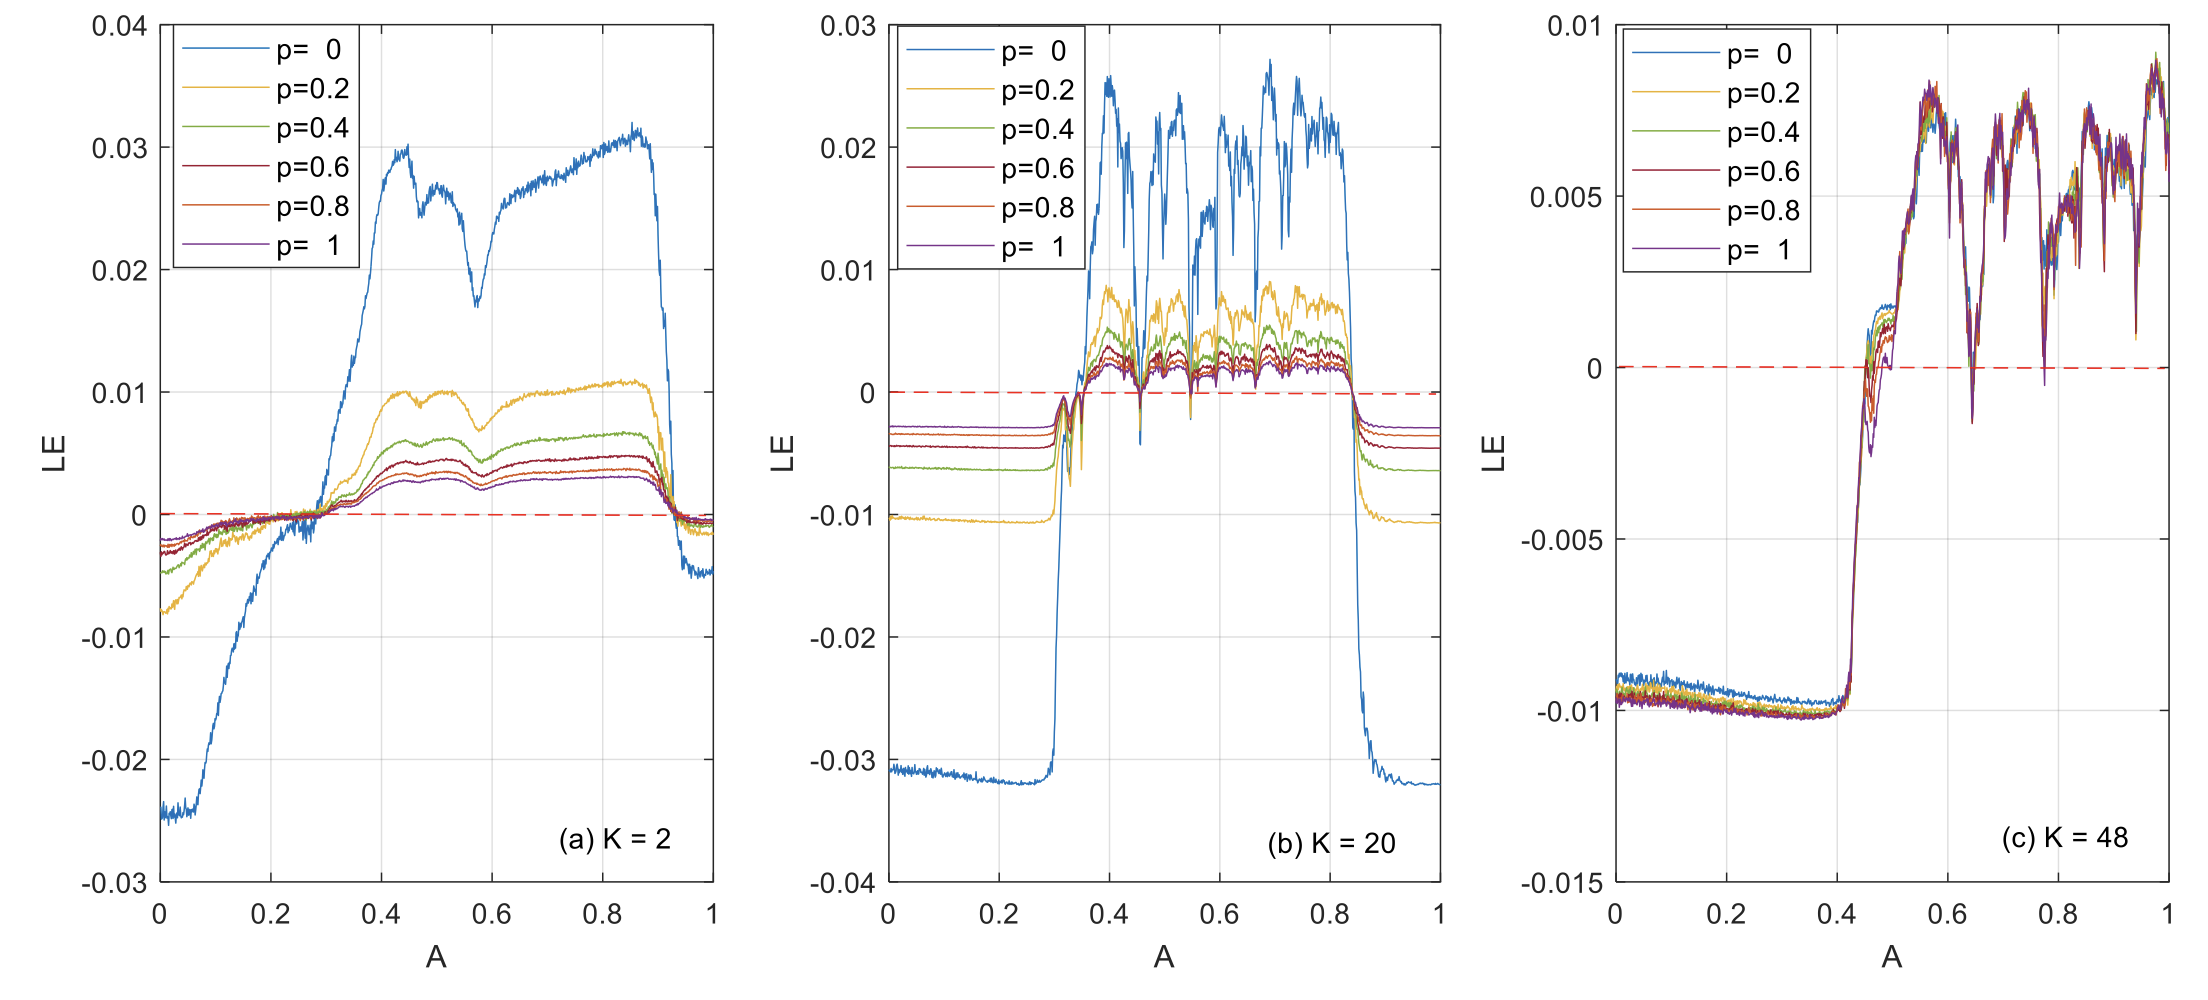
\includegraphics[width=\textwidth]{34.png}
\end{figure}
\subsection{同步性分析}
事实上,大量耦合粒子的同步化问题最早由1998年给出的基于变分方程的主稳定函数方法而得到妥善地解决[*]。下面我们仍然基于变分法给出本章所提Duffing-WS小世界网络(*)的主稳定函数,并由此分析Duffing-WS小世界网络的同步性。
Duffing-WS小世界网络的变分方程已由(*)式给出,令
\begin{eqnarray*}
\boldsymbol{\delta}_{i}=\left[\delta_{xi}, \delta_{yi}, \delta_{zi}\right]^T,
\end{eqnarray*}
则Duffing-WS 小世界网络的变分方程(*)可以简化为如下的矢量形式:
\begin{equation}
    \dot{\boldsymbol{\delta}}_i=D f(\mathbf{S}) \boldsymbol{\delta}_i-c \sum_{j=1}^N l_{i j} H \boldsymbol{\delta}_j, i=1,2, \ldots, N
\end{equation}
其对应的孤立节点动力学函数为
\begin{eqnarray*}
 f(\mathbf{X})=\left[\begin{array}{c}y \\ -\gamma y+a x-b x^3+A \sin (z) \\ \Omega\end{array}\right],
\end{eqnarray*}
节点内连矩阵为:
\begin{eqnarray*}
H=\left[\begin{array}{lll}
0 & 0 & 0 \\
1 & 0 & 0 \\
0 & 0 & 0
\end{array}\right].
\end{eqnarray*}

令同步流形为 $\mathbf{S}(t)=(s(t), \dot{s}(t), \Omega t)^T$, 即孤立节点动力学方程 $\dot{\mathbf{S}}(t)=f(\mathbf{S})$ 的解。
$D f(\mathbf{S})$ 则为单节点动力学函数在同步流形 $\mathbf{S}(t)=(s(t), \dot{s}(t), \Omega t)^T$ 处的雅可比矩阵, 有
\begin{equation}
    D f(\mathbf{S})=\left[\begin{array}{ccc}
    0 & 1 & 0 \\
    a-3 b s^2(t) & -\gamma & A \cos (\Omega t) \\
    0 & 0 & 0
    \end{array}\right]
\end{equation}
令 $\boldsymbol{\delta}=\left(\boldsymbol{\delta}_1, \ldots, \boldsymbol{\delta}_N\right)$, 则(3.11)式可以改写为
\begin{equation}
    \dot{\boldsymbol{\delta}}=D f(\mathbf{S}) \boldsymbol{\delta}-c H \boldsymbol{\delta} L^T
\end{equation}
不妨假设Laplacian矩阵可对角化 (即为无向图情况)), $L^T=P \Lambda P^{-1}, \Lambda=\operatorname{diag}\left(\lambda_1, \ldots, \lambda_N\right)$, 
令 $\boldsymbol{\eta}=\boldsymbol{\delta} P$, 则方程组又等价于如下的方程组:
\begin{equation}
    \begin{gathered}
    \dot{\boldsymbol{\eta}}_1=D f(\mathbf{S}) \boldsymbol{\eta}_1, k=1,2, \ldots, N \\
    \dot{\boldsymbol{\eta}}_k=\left[D f(\mathbf{S})-c \lambda_k H\right] \boldsymbol{\eta}_k, k=2, \ldots, N
    \end{gathered}
\end{equation}
第一式对应于与同步流形平行方向的扰动,为保证同步流形的稳定性,需要第二式描述的$N-1$个子系统是渐近稳定的。注意到除非$s(t)$是平衡点,
否则第二式中的每个子系统都是时变系统,判断同步流形稳定的一个常用判据是要求主稳定方程的所有Lyapunov指数全为负值。
方程组(*)所对应的主稳定方程可以写为:
\begin{equation}
    \dot{\boldsymbol{y}}=\boldsymbol{M}(\alpha)\boldsymbol{y}
\end{equation}
其中 $\boldsymbol{M}(\alpha)=\left[\begin{array}{ccc}0 & 1 & 0 \\ a-3 b s^2(t)-\alpha & -\gamma & A \cos (\Omega t)
\\ 0 & 0 & 0\end{array}\right], \alpha=c \lambda_k$。这里假设主稳定方程的最大李亚普洛夫指数为 $LE(\alpha)$。

将主稳定方程和单个节点的Duffing方程联立,得到
\begin{equation}
    \left\{\begin{array}{l}
    \dot{s}_1=s_2 \\
    \dot{s}_2=-\gamma s_2+a s_1-b s_1^3+A \sin (\Omega t) \\
    \dot{y}_1=y_2 \\
    \dot{y}_2=\left(a-3 b s_1^2-\alpha\right) y_1-\gamma y_2+A \sin (\Omega t) y_3 \\
    \dot{y}_3=0
    \end{array}\right.
\end{equation}
于是,其最大 Lyapunov 指数由下式给出:
\begin{equation}
L E(\alpha)=\lim _{T \rightarrow+\infty}
\frac{\ln \left(\left|y_1(T)\right|+\left|y_2(T)\right|\right)}{T}
\end{equation}

下面的图绘制了当周期驱动幅度$A$在[0,1]范围内时,主稳定方程(*)平面Lyapunov指数的相图,即其最大 Lyapunov指数关于参数$\alpha$和振幅$A$的变化图,
其中黑色区域为最大Lyapunov指数非负即不同步的区域。同样,我们按照不同初始值取了50次平均得到最后的结果。\par
\begin{figure}[!htbp]
    \centering
    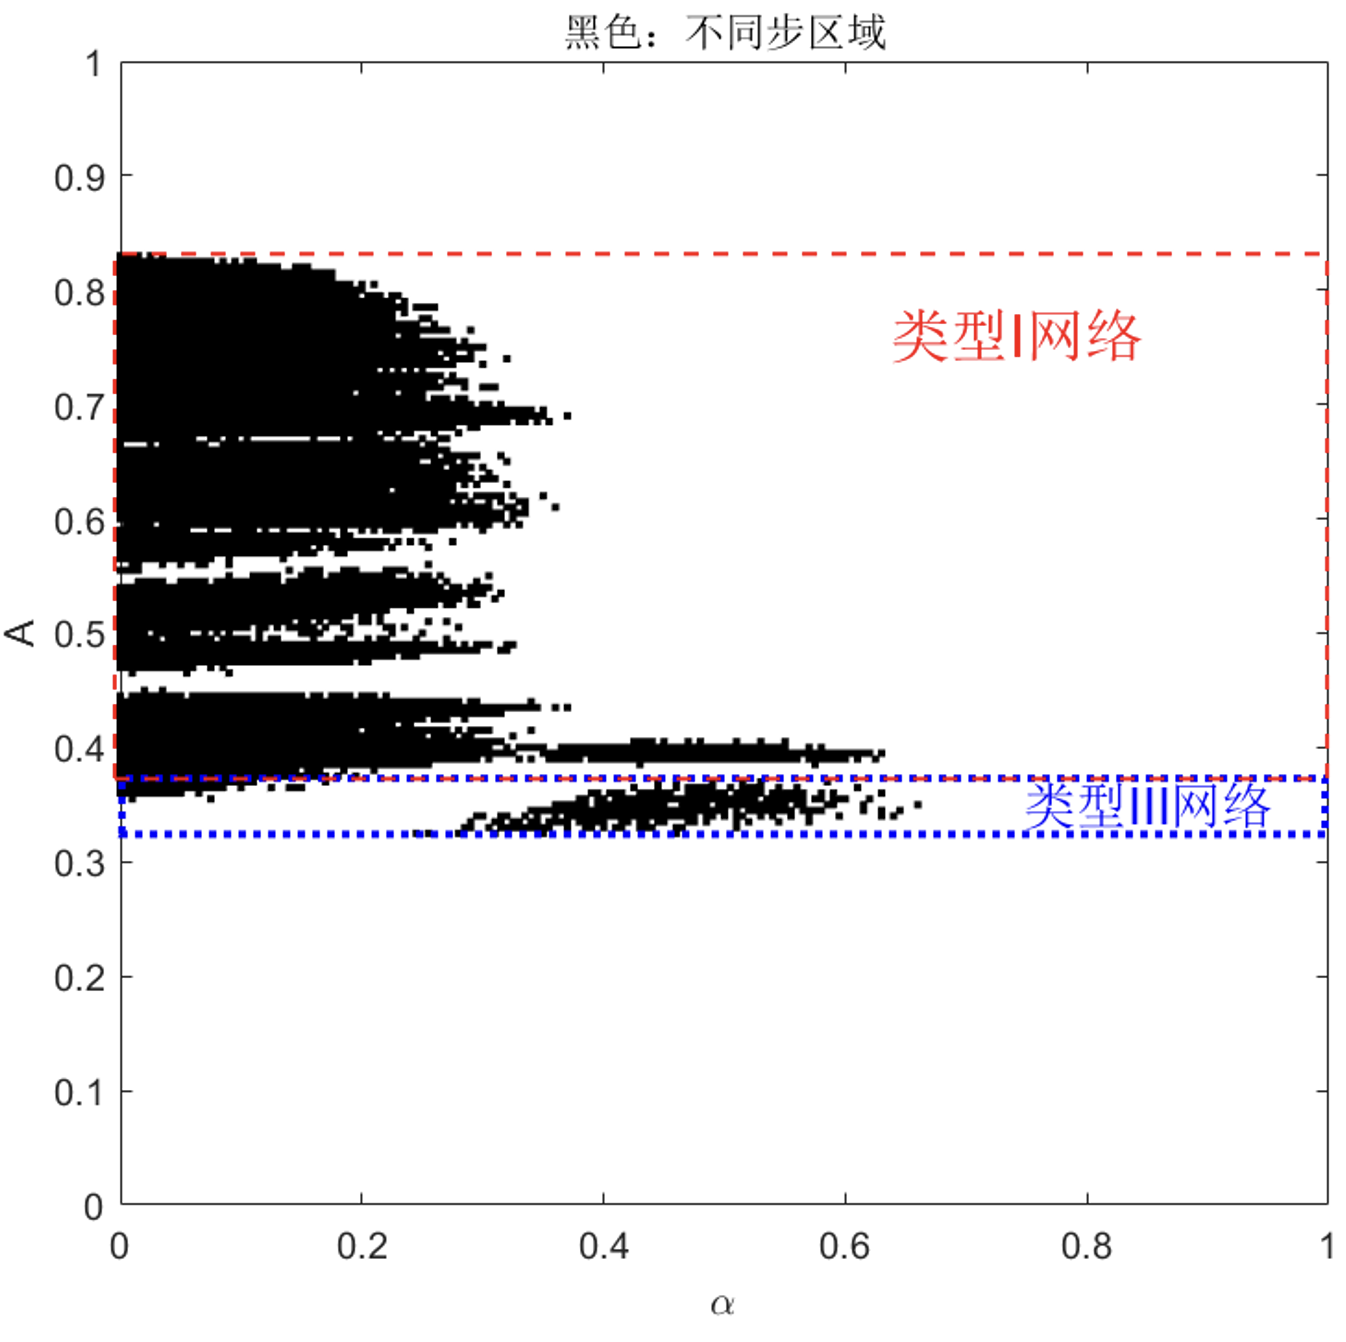
\includegraphics[width=0.8\textwidth]{tb1.png}
\end{figure}
分析图(*),我们可以得出如下结论:

(1)当 $A \in[0,0.32] \cup[0.83,1]$ 时, 主稳定方程的最大 $\mathrm{LE}$ 指数全为负数, 即我们考虑的Duffing-WS小世界网络(*)的同步化区域为全区域 $S R=(0,+\infty)$,
这时候的系统总是可以达到完全同步 (和耦合网络结构小世界特性无关);\par

(2)当 $A \in[0.33,0.37]$ 时, 网络属于类型$\mathrm{III}$的网络, 其同步化区域为不连通的多区域 $S R=\left(0, \alpha_1\right) \cup\left(\alpha_2,+\infty\right)$,
这时候系统要达到完全同步, 必须满足 $c \lambda_k \in S R, k=2,3, \ldots, N$,
而要同时调整耦合强度和所有特征值全部落入不连通的同步化区域 SR。此时,
如果满足 $c \lambda_2>\alpha_2$, 则 $\alpha_2<c \lambda_2 \leq \ldots \leq c \lambda_N$ 时,
都有 $L E(\alpha)<0$, 同步流形总是稳定的, 系统总能同步。

在这种情况下, 网络Laplacian 矩阵的第二大特征值
$\lambda_2$ 的大小可以作为衡量网络同步化能力的指标, $\lambda_2$ 越 大则系统越容易达到同步, 也就是系统的同步化能力越强。
如果 $\alpha_1<c \lambda_2<\alpha_2$, 则同步流形不稳定, 系统不能同步。如果 $c \lambda_2<\alpha_1$,
则要求 $c \lambda_N<\alpha_1\left(\lambda_N / \lambda_2<c\right)$ 或者 $\alpha_2<c \lambda_3$, 则同步流形稳定,
此时系统同步相对于前 面两种情况更不容易实现。

(3)当 $A \in[0.38,0.82]$ 时, 网络属于类型 $\mathrm{I}$ 的网络, 其同步化区域为无界区域 $S R=\left(\alpha_3,+\infty\right)$,
即当 $\alpha_3<c \lambda_2 \leq \ldots \leq c \lambda_N$ 时, 都有 $L E(\alpha)<0$, 即 $c \lambda_2>\alpha_3$,
同步流形总是稳定的, 系统总能同步。在这种情况下, Laplacian 矩阵的第二大 特征值 $\lambda_2$ 的大小也是可以作为衡量网络同步化能力的指标。\par

综上可知, 对于不同的 $A$ 值, 当 Laplacian 矩阵的第二大特征值 $\lambda_2$ 和耦合系数的乘积 $c \lambda_2$ 充分大时,
系统总能实现同步; 给定耦合系数 $\mathrm{c}$, Laplacian 矩阵 的第二大特征值 $\lambda_2$ 决定了系统的同步能力,
当 $\lambda_2$ 的值较小时, 系统则很有可能 不能同步。但是当增加耦合系数 $\mathrm{c}$ 大于某个值时, 对于系统也总能实现同步。

下图给出了粒子个数为 $\mathrm{N}=20,100$ 时, Duffing-WS小世界网络 Laplacian 矩阵的第二大特征值 $\lambda_2$在不同的 $\mathrm{K}$ 值下随重连概率 $\mathrm{p}$
变化的曲线(平均 100次)。可以看到当连接度较小 $(\mathrm{K}=1)$时, 第二大特征值 $\lambda_2$ 随着重连概率增加先减小后增加,
说明此时较小或较大的重连概率均有利于增加系 统同步; 随着连接度增加(左图, $K=2,3,4,5,6$ ), 第二大特征值 $\lambda_2$
随着重连概率增加先增加后减小, 说明此时适当大小的重连概率有利于增加系统的同步; 当连接 度继续增加而接近 $\mathrm{N} / 2$ 时,
第二大特征值 $\lambda_2$ 随着重连概率增加而减小, 说明较小的重连概率有利于增加系统的同步。\par
\begin{figure}[!htbp]
    \centering
    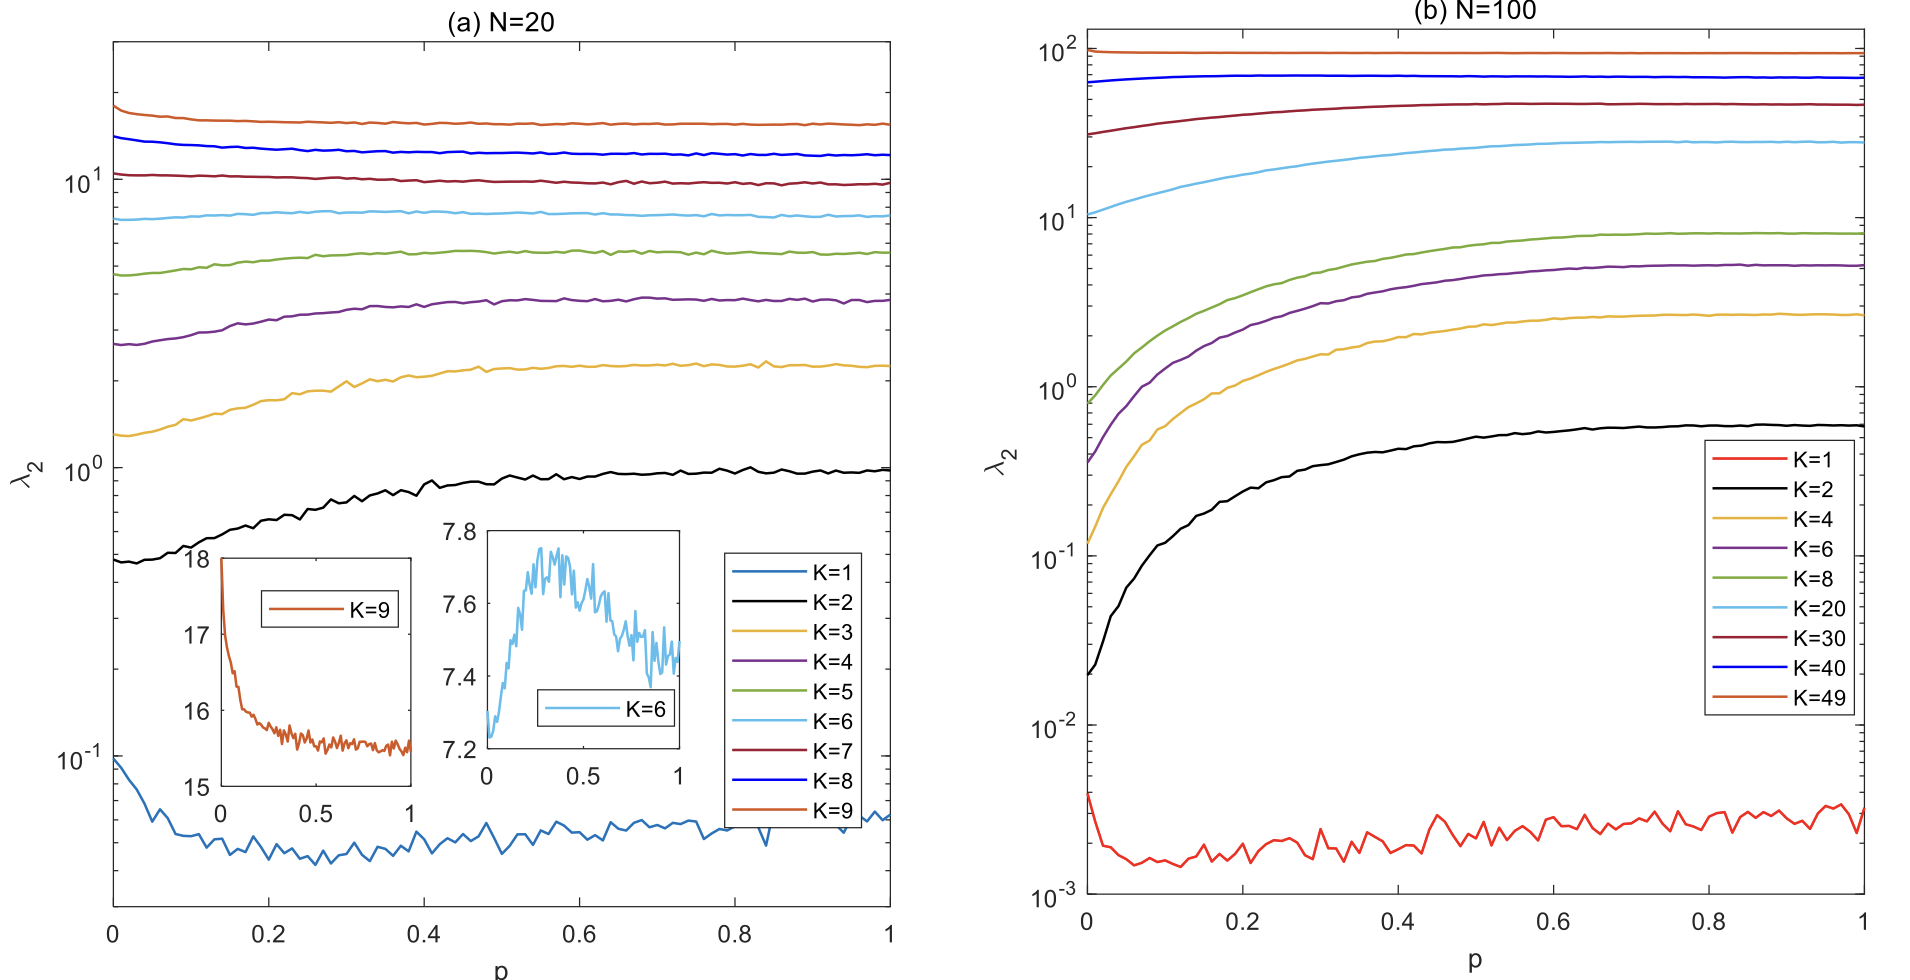
\includegraphics[width=\textwidth]{tb2.png}
\end{figure}
下图则给出了粒子个数为 $\mathrm{N}=20,100$ 时, Duffing-WS小世界网络 Laplacian 矩阵的最大特征值 $\lambda_N$在不同的 $\mathrm{K}$ 值下随重连概率 $\mathrm{p}$
变化的曲线(平均 100次)。
\begin{figure}[!htbp]
    \centering
    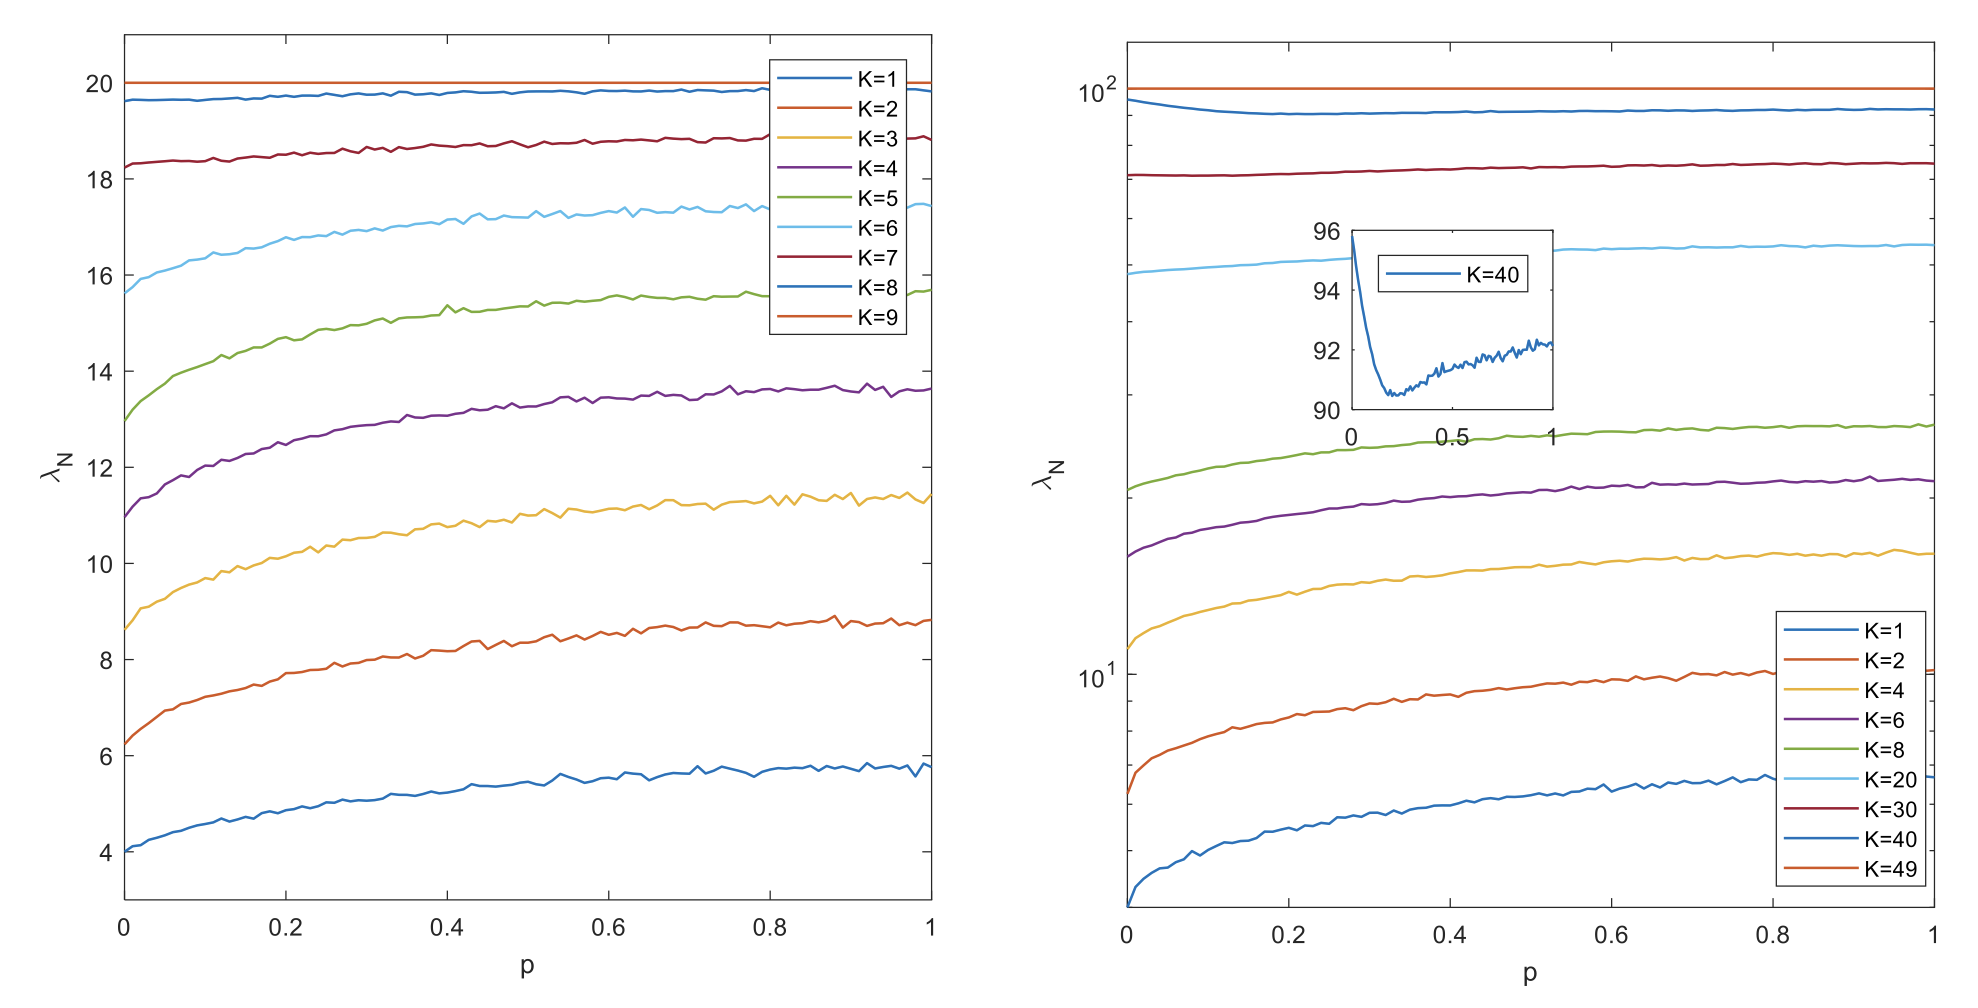
\includegraphics[width=\textwidth]{tb3.png}
\end{figure}
\section{小结} 
本文基于经典的Duffing振子,提出了一个以WS小世界网络方式进行连接的Duffing型复杂网络
(简称Duffing-WS型小世界网络),利用变分法推导该网络的最大李雅普诺夫指数表达式,
以庞加莱截面分岔图和李雅普诺夫指数为工具研究其混沌现象,并分析小世界网络重连度,
重连概率和耦合强度等参数对其混沌运动状态参数范围的影响。研究表明,Duffing-WS小世界网络的各
个粒子输出也呈现出小尺度周期运动、倍周期分岔、混沌和大尺度周期运动等多种状态,
其混沌的参数范围较单个Duffing方程更为复杂。网络重连度,重连概率和耦合强度等参数对其混
沌区域的影响也较传统规则网络有明显不同。